% \documentclass{book}

\documentclass[12pt]{article}
\usepackage[pdfborder={0 0 0.5 [3 2]}]{hyperref}%
\usepackage[left=1in,right=1in,top=1in,bottom=1in]{geometry}%
\usepackage[shortalphabetic]{amsrefs}%
\usepackage{amsmath}
\usepackage{enumerate}
\usepackage{enumitem}
\usepackage{amssymb}                
\usepackage{amsmath}                
\usepackage{amsfonts}
\usepackage{amsthm}
\usepackage{bbm}
\usepackage[table,xcdraw]{xcolor}
\usepackage{tikz}
\usepackage{float}
\usepackage{booktabs}
\usepackage{svg}
\usepackage{mathtools}
\usepackage{cool}
\usepackage{url}
\usepackage{graphicx,epsfig}
\usepackage{framed}
\usepackage{hyperref}  

\graphicspath{ {images/} }

\def\noi{\noindent}
\def\T{{\mathbb T}}
\def\R{{\mathbb R}}
\def\N{{\mathbb N}}
\def\C{{\mathbb C}}
\def\Z{{\mathbb Z}}
\def\P{{\mathbb P}}
\def\E{{\mathbb E}}
\def\Q{\mathbb{Q}}
\def\ind{{\mathbb I}}

\begin{document}

\title{}
\author{\vspace{-10ex} }

\begin{center}
{\LARGE APMA 1650 -- Homework 3}\\
\vspace{5mm}
{\large Due Monday, July 11, 2016}\\
\vspace{5mm}
Homework is due during class or by 3:45 pm in the homework drop box in 182 George St.\\
Show all of your work used in deriving your solutions.
\end{center}

\begin{enumerate}

\item Two people are playing a game. They take turns rolling a standard, fair six-sided die. The game ends when one player rolls a 6. The player who rolls the 6 is the winner of the game. A ``round'' of the game is defined as a single die roll.
\begin{enumerate}
\item What is the probability that the player who goes first wins?\\

Let $S$ be the event that a 6 is rolled, and $N$ the event that a 6 is not rolled. We can represent each game as a string of 0 or more Ns followed by a single S. For the first player to win, the game must last an \emph{odd} number of rounds, so one of the following game strings must occur:
\begin{figure}[H]
\centering
\begin{tabular}{l@{\hskip 2cm}l}
\toprule
String & Probabiltiy\\
\midrule
S & $1/6$\\
NNS & $(5/6)^2 (1/6)$ \\
NNNNS & $(5/6)^4 (1/6)$\\
$\vdots$ & $\vdots$\\
\bottomrule
\end{tabular}
\end{figure}
To find the probability that the first player wins, we sum the probabilities in the right hand column above:
\begin{align*}
\P(\text{Player 1 wins}) = (1/6) + (1/6) (5/6)^2 + (1/6) (5/6)^4 +  (1/6) (5/6)^6 + \cdots
\end{align*}
This is a geometric series with first element $1/6$ and common ratio $(5/6)^2 = 25/36$. Thus the probability that the first player wins is the sum of this geometric series.
\begin{align*}
\P(\text{Player 1 wins}) = \frac{1/6}{1 - 25/36} = \frac{1/6}{11/36} = \frac{6}{11}
\end{align*}
This is slightly greater than 1/2, so if you are playing this game, you want to go first.

\item What is the expected value and variance for the number of rounds in the game?\\

Here we do not care who win, just how long the game lasts. Let $X$ be the number of rounds the game lasts. Since we are rolling a die repeatedly until we roll a 6, this is a geometric distribution, with ``success'' defined as rolling a 6. Since the probability of rolling a 6 is $p = 1/6$, then $X \sim$Geometric(1/6). We can look up the expected value and variance of the geometric distribution to get:
\begin{align*}
\E(X) &= \frac{1}{p} = \frac{1}{1/6} = 6 \\
Var(X) &= \frac{1-p}{p^2} = \frac{5/6}{1/36} = 30
\end{align*}

\item What is the probability that the game lasts at least 4 rounds?\\

Using our geometric random variable $X$, we want $\P(X \geq 4)$. We could compute $\P(X < 4) = \P(X = 1) + \P(X = 2) + \P(X = 3)$ and subtract from 1. Or we could note that the game lasting at least 4 rounds is equivalent to ``failure'' on the first 3 rounds, i.e. not rolling a 6 on the first 3 rounds. So
\[
\P(X \geq 4) = \P(\text{``failure'' on first 3 rounds}) = (1 - p)^3 = (5/6)^3
\]

\item Given the game has lasted four rounds, what is the probability that the game lasts at least 8 rounds?\\

The probability that the game lasts at least 8 rounds given that it has lasted 4 is $\P(X \geq 8 | X \geq 4)$. Using the definition of conditional probability, and noting that if a game lasts at least 8 rounds it has also lasted at least 4 rounds:
\[
\P(X \geq 8 | X \geq 4) = \frac{ \P(X \geq 8 \cap X \geq 4) }{ \P(X \geq 4) } = \frac{ \P(X \geq 8 ) }{ \P(X \geq 4) }
\]
Using part (c), and extending it to the case where the game lasts at least 8 rounds, we have:
\[
\P(X \geq 8 | X \geq 4) = \frac{ (1 - p)^7  }{ (1 - p)^3 } = (1-p)^4 = (5/6)^4
\]
\end{enumerate}

\item A single cell will die with probability $p$ or split into two cells with probability $1 - p$, producing a second generation of cells. Each cell in the second generation (if there are any) will die or split into two with the same probabilities as the initial cell. You start with a single cell.
\begin{enumerate}
\item Find the probability mass function (pmf) for the number of cells in the third generation.\\

To find the probability mass function, we can first draw a tree diagram to see what is happening.
\begin{figure}[H]
\centering
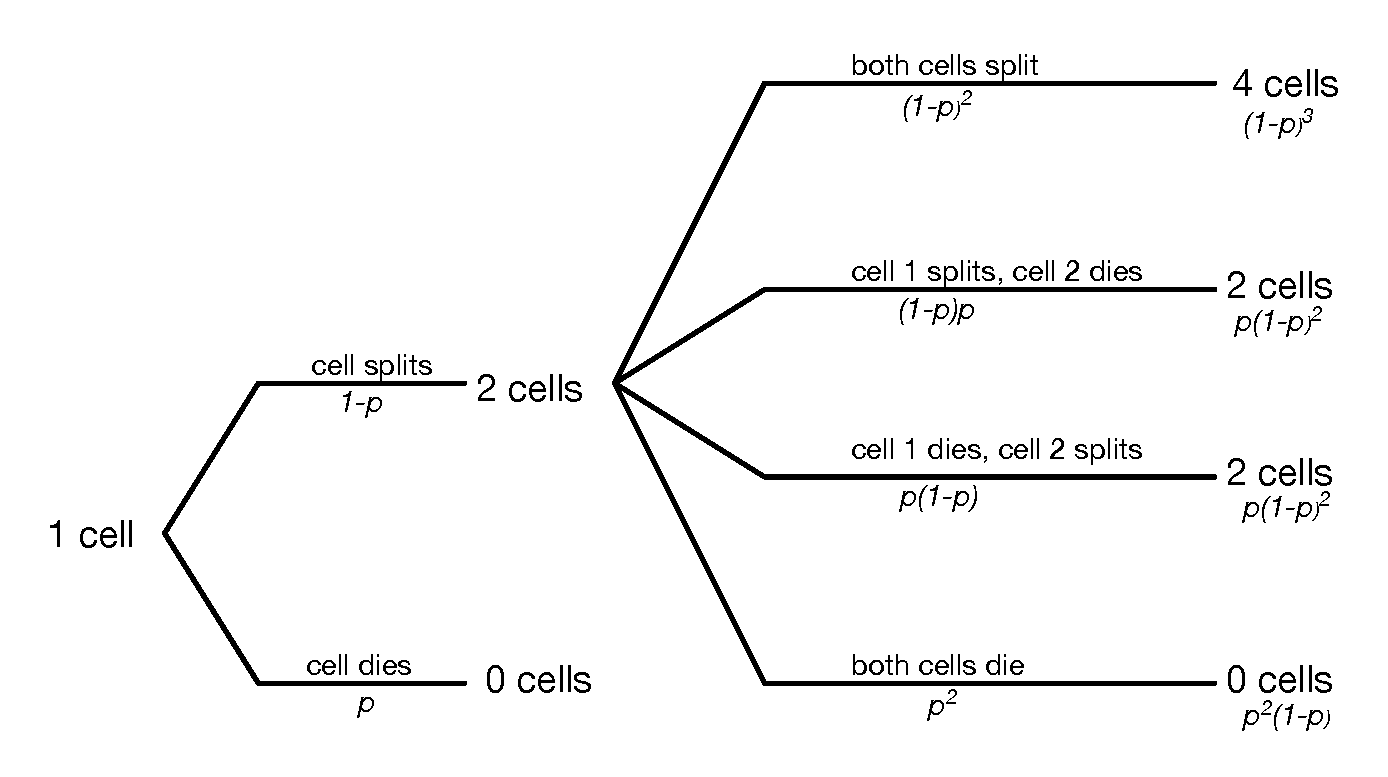
\includegraphics[width=10cm]{celltree.eps}
\end{figure}
Using the tree, we can write the pmf in a table. There are two branches in the tree which lead to 2 cells and two branches in the tree which lead to 0 cells. Don't forget to add them together! Let $Y$ be the number of cells in the 3rd generation. Then we have the following pmf for $Y$.
\begin{figure}[H]
\centering
\begin{tabular}{l@{\hskip 2cm}l}
\toprule
$y$ & $p(y)$\\
\midrule
0 & $p + p^2(1-p)$\\
2 & $2p(1-p)^2$ \\
4 & $(1-p)^3$\\
$\vdots$ & $\vdots$\\
\bottomrule
\end{tabular}
\end{figure}

\item What is the expected value of the number of cells in the third generation?\\

Using the pmf table above and the formula for the expected value of a discrete random variable:
\begin{align*}
\E(Y) &= 0 \cdot (p + p^2(1-p)) + 2 \cdot 2p(1-p)^2 + 4 \cdot(1-p)^3 \\
&= 4 p(1-p)^2 + 4 (1-p)^3 \\
&= 4(1-p)^2(p + (1-p)) \\
&= 4(1-p)^2
\end{align*}
\end{enumerate}

\item When you are not studying for APMA 1650, you work part-time as a barista at a local coffee shop. Customers arrive at your coffee shop at an average rate of 10 customers per hour.
\begin{enumerate}
\item Model this problem with an appropriate probability distribution. What is the probability that fewer than 5 customers arrive in a fixed, one-hour period?\\

Since we have events occurring with a constant average rate in a fixed span of time, and the events occur independently from each other (or at least roughly: two friends could come into your coffee shop together), we will model this with a Poisson distribution with parameter $\lambda = 10$. Let $X \sim$Poisson(10). Then:
\begin{align*}
\P(X < 5) &= \P(X = 0) + \P(X = 1) + \P(X = 2) + \P(X = 3) + \P(X = 4)\\
&= \frac{e^{-10} 10^0}{0!} + \frac{e^{-10} 10^1}{1!} + \frac{e^{-10} 10^2}{2!} + \frac{e^{-10} 10^3}{3!} + \frac{e^{-10} 10^4}{4!}\\&\approx 0.029
\end{align*} 
Don't forget that a Poisson random variable can take the value 0.

\item What is the probability that 5 or more customers arrive in a fixed, one-hour period?\\
This is the complementary event from part (a), so we subtract from 1 to get $\P(X \geq 5) = 1 - \P(X < 5) \approx 1 - 0.029 = 0.971$.

Suppose it takes 4 minutes to serve one customer. The total service time is the number of minutes during a fixed, one-hour period which are spent serving customers.
\item What is the average total service time?\\

The total service time is just the number of customers multiplied by 4. Let $Y$ be the total service time. Then $Y = 4X$. Using linearity of expectation,
\[
\E(Y) = \E(4X) = 4\E(X) = 4(10) = 40
\]
where we used the fact that the expected value of a Poisson random variable is its parameter $\lambda$, which is 10 in this problem.

\item What is the variance of the total service time?\\
Here we use the expression $Var(aX + b) = a^2 Var(X)$.
\[
Var(Y) = Var(4X)= 4^2 Var(X) = 16(10) = 160
\]
where we used the fact that the variance of a Poisson random variable is also its parameter $\lambda$
\end{enumerate}

\item A particular flight can only fit 200 people, but tickets were sold to 205 people. Suppose each ticket holder has a 0.05 probabiltiy of not showing up for the flight.
\begin{enumerate}
\item What is the probability that the flight will be overbooked? Give an approximate numerical answer for this.\\

We can model this problem with a binomial distribution, since we have $n = 205$ customers, each of whom has (independently) a $p =0.95$ probabiltiy of showing up. (Again, think of whether this is realistic; if a family travels together, then it is likely that they will either all show up or all not show up, so we might not have complete independence; however, in this case, it is good enough for our purposes). Defining ``success'' as showing up for the flight, let $X \sim$Binomial(205, 0.95). The probability that the flight will be overbooked is:
\begin{align*}
\P(X > 200) &= \P(X = 201) + \P(X = 202) + \P(X = 203) + \P(X = 204) + \P(X = 205) \\
&= \binom{205}{201} 0.95^{201} 0.05^4 +  \binom{205}{202} 0.95^{202} 0.05^3 + \binom{205}{203} 0.95^{203} 0.05^2 \\
&\:\:\:\:\:+ \binom{205}{204} 0.95^{204} 0.05^1 + \binom{205}{205} 0.95^{205} 0.05^0 \\
\approx 0.022   
\end{align*}
So it is highly unlikely that the flight will be overbooked.

\item What is the expected number of people that show up for the flight?\\

Using the formula for the expected value of a binomial random variable:
\[
\E(X) = np = 205(0.95) = 194.75
\]
\item What is the variance of the number of people who show up for the flight?\\

Using the formula for the variance of a binomial random variable:
\[
\E(X) = np(1-p) = 205(0.95)(0.05) = 9.7375
\]
\end{enumerate}

\item You reprise your role as the quality control manager for the Acme Widget Company. You have found that in every box of 100 widgets there is on average 1 defective widget.
\begin{enumerate}
\item Model this problem with an appropriate probability distribution. What is the probability that a box of 100 widgets contains 2 or fewer defective widgets?\\

Defining ``success'' as finding a defective widget, since we are looking for the number of successes out of $n =100$ Bernoulli trials, we can model this with a Binomial random variable. The probabiltiy of finding a defective widget is $p = 1/100 = 0.01$. Let $X\sim$Binomial(100, 0.01). Then
\begin{align*}
\P(X \leq 2) &= \P(X = 0) + \P(X = 1) + \P(X = 2) \\
&= \binom{100}{0}0.01^0 0.99^{100} + \binom{100}{1}0.01^1 0.99^{99} + \binom{100}{2}0.01^2 0.99^{98}\\
&\approx 0.920627
\end{align*}
\item Approximating this with a Poisson distribution, find the probability that you have 2 or fewer defective widgets.\\

We need a Poisson random variable with the same mean as the Binomial random variable in (a). Using the formula for the expected value of a Binomial random variable, $\E(X) = np = (100)(0.01) = 1$. Let $Y \sim$Poisson(1).
\begin{align*}
\P(Y \leq 2) &= \P(Y = 0) + \P(Y = 1) + \P(Y = 2) \\
&= \frac{e^{-1} 1^0}{0!} + \frac{e^{-1} 1^1}{1!} + \frac{e^{-1} 1^2}{2!}\\
&\approx 0.919699
\end{align*}

\item Evaluating both part (a) and part (b) numerically using Wolfram Alpha or your favorite software package, what is the relative error for your Poisson approximation\footnote{relative error is $|$true value - approximate value$|$ / true value}?\\

We computed the approximate values above. They look pretty close. How close are they?
\[
\text{Relative error} = \frac{ |0.920627 - 0.919699| }{0.919699} \approx 0.001
\]
So the Poisson approximation is accurate within 0.1\%, which is fantastic.
\end{enumerate}

\end{enumerate}

\end{document}

